\documentclass[conference]{sig-alt-gov2}
\pdfpagewidth=8.5in
\pdfpageheight=11in
%\usepackage{subfig}
\usepackage{subfigure}
\usepackage[pdftex]{}
\usepackage{todonotes}
\usepackage{listings}
\lstset {% general command to set parameter(s)
         language=C,
     basicstyle=\footnotesize,               % print whole listing small
%     keywordstyle=\color{black}\bfseries, % underlined bold black keywords
%     identifierstyle =\color{black},  % nothing happens
%     commentstyle=\color{black}\emph, % white comments
     %stringstyle=\ttfamily,          % typewriter type for strings
%     stringstyle=\color{black},       % typewriter type for strings
         tabsize=4,
         showtabs=false,
     showstringspaces=false}
%can't figure this one out for particles bandwidth
%\usepackage[caption,label]{subfig}

%\newcommand{\TITLE}{D\textsuperscript{\huge{2}}T: Doubly Distributed Transactions for High Performance and Distributed Computing}

\newcommand{\DDT}{D\textsuperscript{2}T~}
\newcommand{\DDTns}{D\textsuperscript{2}T}

\hyphenation{sub-trans-ac-tion}

% in order for balance columns to work, it has to be before begin document...
%\balancecolumns

\begin{document}

\conferenceinfo{MSST'14,} {November 17, 2013, Denver, Colorado, USA.}
\CopyrightYear{2014}
%\crdata{978-1-4503-1103-8/11/11}
\clubpenalty=10000
\widowpenalty = 10000

\title{Considerations for the Next Iteration of the DOE Fast Forward Storage and IO Project}

\numberofauthors{3}
\author{
\alignauthor Jay Lofstead\\
       \affaddr{Sandia National Laboratories}\\
       \email{gflofst@sandia.gov}
\alignauthor Ivo Jimenez\\
       \affaddr{University of California, Santa Cruz}\\
       \email{ivo@cs.ucsc.edu}
\alignauthor Carlos Maltzahn\\
       \affaddr{University of California, Santa Cruz}\\
       \email{carlosm@soe.ucsc.edu}
%\and  % use '\and' if you need 'another row' of author names
}
\maketitle

\begin{abstract}
With phase 1 of the Fast Forward Storage and IO Stack project complete, it is
an excellent opportunity to evaluate many of the decisions made to feed into
the phase 2 effort. The initial effort to define a next generation filesystem
has made admirable contributions in architecture and design. Formalizing the
general idea of data staging as burst buffers for the file system will help
manage the performance variability and offer the data processing opportunities
outside the main compute and file system. Adding a tranasctional mechanism to
manage faults and data visilibilty helps enable effective analytics without
having to work around the IO stack semantics.

While these and other their contributions are valuable, similar efforts made
elsewhere may offer attractive alternatives or differing semantics that would
yield a more feature rich environment with little to no additional overhead.
For example, the Doubly Distributed Transactions (\DDTns) protocol offers an
alternative approach for incorporating transactional semantics into the data
path. The PreDatA project examined how to get the best throughput for data
operators can offer some insights for refining the Burst Buffer concept.

This paper examines some of the choices made by the FastForward team and
compares them with other options and offers observations and suggestions based
on these other efforts.  This will include some non-core contributions of other
projects, such as some of the demonstration metadata and data storage
components generated while implementing \DDTns, to make suggestions that may
help the next generation design for how the IO stack works as a whole.

\end{abstract}

\category{D.4}{Software}{Operating Systems}
\category{D.4.7}{Operating Systems}{Organization and Design}[hierarchical design]

\terms{Design, Performance}

\section{Introduction}

Current production HPC IO stack design is unlikely to offer sufficient features
and performance to adequately serve the needs of an extreme scale platform. To
address these limitations, the US Department of Energy commissioned an effort
to develop a design and prototype for an IO stack suitable for the extreme
scale environment. This is a joint effort led by the Intel Lustre team, Los
Alamos National Laboratory, EMC, and the HDF Group. This team has developed a
specification set~\cite{fastforward:2014:docs} for a future IO stack to address
the identified challenges. The first phase recently completed with a second
phase getting underway. The core focus of the first phase was basic
functionality and design. The second phase will refine this design
incorporating fault recovery and other features missing from the first phase.

The basic architecture incorporates five layers. The top layer is a high level
IO library, such as the demonstration HDF-5 library. The intent is to only have
access to the storage stack through such an API to manage the complexity of
working with the lower layers. Below the user API is an IO forwarding layer
that redirects IO calls from the compute nodes to the IO dispatching layer.
This IO forwarding layer is analogous to the function of the IO nodes in a
BlueGene machine. The next two layers have considerable functionality. The IO
dispatcher (IOD) serves as the primary storage interface for the IO stack and
is the only way to reach the persistent storage array in lower layers.

The core idea for IOD is to provide a way to manage the IO load that is
separate from the compute nodes and the storage array. Communication intensive
acitivies, such as two-phase, data sieving IO's data rearrangement process, can
be moved to the IOD layer offloading the communication load from the compute
nodes. IOD has three main purposes. First, if the optional burst buffer is
availble, it works as a fast cache absorbing write write operations for the
slower trickle out to the central storage array. It can also be used to
retrieve objects from the central storage array for more efficient read
operations and offer data filtering to make client reads more efficient.
Second, it offers the transaction mechanism for controlling data set visibility
and to manage faults that should prevent a data set from being used. Third,
data processing operations can be placed in the IOD. This operations are
inteded to offer data rearrangement, filtering, and similar operations prior to
it reaching the central storage array.

Offloading the collective two-phase data sieving from the compute nodes to
reorganize data has proven effective at reducing the total time for writing
data due to fewer participants involved in the communication
patterns~\cite{lofstead:2011:nessie-staging}.  Beyond these broad items, there
are many important details some of which are examined in more detail below.

The bottom two layers are the Data Access Object Storage (DAOS) and Versioning
Object Storage Device (VOSD). DAOS is the typical interface that represents
the individual objects stored including the semantics related to ``files''.
VSOD is the actual storage mechanism for the objects defined at the DAOS layer.

The focus of this paper is primarily the IOD layer given the critical role it
has in the performance and functionality of the entire stack. Most of the key
features explored in this paper all have a strong presence in the IOD layer
motivating the focus of this examination.

%Incorporated into the design of these layers and the function of some of these
%layers themsleves, such as the IOD layer, are features to manage both burst IO
%performance and faults. In particular, the IOD layer's use of burst buffers
%attempts to absorb a massive data dump from the compute area that is then
%trickled to the persistent storage area only if desired. Otherwise, it can be
%stored locally on optional SSDs for use by analysis routines eliminating the
%need to use slower rotational media as the intermediary between a simulation
%and the analysis code.

%A second feature is the incorporation of a transaction like mechanism into the
%IOD layer and a related epochs feature into the DAOS layer. This feature offers
%a mechanism to avoid making incomplete data visible to other users and offer a
%level of protection if the data can be stored on the optional SSDs. The
%implications of how these concepts are designed are important to consider for
%the final design. Because they control data visibility and manage faults for
%output operations, they are key features.

The rest of the paper is organized as follows. Section~\ref{sec:burst}
discusses some of the features of incoporating burst buffers as designed and
suggests some considerations and alternatives for the next generation of this
project. Section~\ref{sec:transactions} discusses the transactions approach
offered in the IOD layer and the corresponding epochs in the DAOS layer. It
also offers a comparison to the \DDT system given the very similar high-level
design and motivating use case.  Section~\ref{sec:optimizations} discusses some
of the optimizations offered by the current design and how and when these
optimizations will work best. It also explores some of the dark corners that
may yield performance issues with the current design. 
Section~\ref{sec:summary} disucsses the system overall with recommendations on
what design elements should be considered based on broader issues with current
HPC data centers. The paper is conclued in Section~\ref{sec:conclusion} with
a summary of the broad issues covered in the paper.

\section{Burst Buffers}
\label{sec:burst}

The idea of burst buffers were initially explored in the context of data
staging~\cite{abbasi:2007:datatap,Abbasi:2009:datatap,nisar:2008:staging,zheng:2010:predata}.
These initial designs all use extra compute nodes to represent the data storage
buffer given the lack of any hardware support for this functionality. The
desired outcome of these initial studies is to motivate how such functionality
might be incorporated and the potential benefits.  Later, these concepts were
proposed to be incorporated as part of the IO
stack~\cite{bent:2012:challenges,bent:2012:burst-buffer}.  The current
FastForward IOD design recommends incorporating SSDs, but specifically lists
these devices as optional. Unfortunately, both incorporating burst buffers and
the use of SSDs in the IOD layer may be problematic.  First, with these burst
buffers being optional, the semantics of how IOD works must change to use DAOS
to store the data directly rather than storing them locally until explicitly
persisted by the user. The design of DAOS does not incorporate a high
transaction rate mechanism. Conversely, it assumes that it will only be
involved when persisting a completed transaction and only for a fraction of the
total transactions created. Further, with function shipping offering the
ability to change how the data is stored and arranged prior to it being written
to DAOS, this functionality may also be optional depending on the existence of
the burst buffer. Consider the important functionality of data rearrangement
and doing things like changing the fast array dimension.

One of the bigger concerns is the observation that the original data staging
proposals all used compute nodes while the newer proposals seek not only to
make them a fixed portion of the IO stack, but also shared across all machine
users. The PreDatA paper in particular examines the potential costs and
advantages of where to place operators similar to the IOD proposed function
shipping. There are two key takeaways from that work. First, placement matters.
Depending on the communication intensity vs. computation intensity, where
along the IO path to place the operation can matter significantly. Second, and
more importantly, the amount of time spent processing for the operators was
stretched to the point where it consumed nearly all of the time between IO
operations. The given ratios of compute processes to staging process examined
is representative for future extreme scale platforms. If anything, the ratios
offer more staging processes than IOD processes would be available.

By concentrating this functionality into the storage stack, three problems
arise.  First, the amount of network bandwidth, IO bandwidth, and compute power
consumed for example operations from a single application is likely to
completely monopolize the IOD processes. Second, if space and time partitioning
is used instead, the functionality risks being too small to be useful. Third,
the hardware performance advantage for SSDs is questionable. Current NAND-based
flash devices top out at around 400 MB/sec. The key spec that is missing from
this number is that 400 MB/sec is a measure of the fixed number of available
IOPS multipled by the block size. This represents the ideal streaming
performance possible. The problem is that it costs an IOP to read 1 byte or 1
block (4KB or 8KB, depending on the device). It costs 1 IOP to write a full
block--usually. In some cases, it will cost 2 IOPs.  This accounts for the
required pre-erase write prior to writing to a reused block. In the worst case,
it can be 3 IOPS per write. This would be for a partial block write (read the
old block, erase, write the modified block). One-third of 400 MB/sec, about 133
MB/sec, is well below the streaming performance of HDDs.  Granted, there is
still rotational and seek latency to deal with for HDDs, but the advantage for
SSDs has evaporated and potentially turned into a penalty at a considerable
cost premium.  There are faster SSD solutions on the market that incorporate
DRAM for caching and using the PCIe bus, for example, but their price precludes
them from use in an extreme scale platform.

Given these features, the optionality and even incorporation of burst buffers
in the current design should be carefully considered. Much of the advanced, key
functionality proposed as they are currently designed ultimatey relies on the
existence of burst buffers to work. Further thought about how to have an IOD
layer both with and without a burst buffer is required before they can be
considered optional. As the design stands today, they are a required part of
the IOD layer for proper functioning. Unfortunately, it is not clear that they
can address the performance concerns they are intended to cover.

\section{Transactions and Epochs}
\label{sec:transactions}

The transaction mechanism manifests in two forms. At the IOD layer, they are
called transactions and are used to judge whether or not an output is complete
or not and control access through treating the transaction ID as a version
identifier. At the DAOS layer, they are called epochs and represent persisted
(durable) transactions from the IOD layer. Each of these offers different
functionality, but are connected as is explained below. How these differ from
the \DDT approach is also explored. While IOD's and \DDTns's transactions are
seemingly very different, they use a similar high-level design, but very
different implementation, to solve the same problem.

\subsection{IOD Transactions}
To understand how transactions are used in the IOD layer, some terminology and
concepts must be explained first. At the coarsest grain level is a container.
Each container serves to host a transaction and contains a collection of
objects. Conceptually, containers corresponds to a file in a traditional file
system. The objects in each container represent different data within a file.
The three initially defined object types are key-value store, array shard,
and blob. The easiest way to understand these types is to evaluate these from
the perspective of an HDF-5 file, the initial user interface layer. The
key-value store represents a collection of attributes. The array shard
represents part of a potentially multi-dimensional array. It is refered to as a
shard because it is likely a small piece of a globally defined array. The blob
represents a byte stream of arbitrary contents.  The fundamental difference
between an array shard and a blob is that the array shard has metadata
identifying its portion within the global, logical space while the blob is
simply a 1-dimensional array of bytes that is not shared across IOD nodes.
Should an operation be deployed into IOD to manipulate an array within a
container, it would operate on the array shards rather than on blobs. Given
this context, the transactions come in two forms.

First is a single leader transaction where the IOD manages based on calls from
a single client. The underlying assumption is that the client side will manage
the transactional operations itself and the single client is capable of
reporting to the IOD how to evolve the transaction state. 

The second form is called multi-leader and has the IOD layer manage the
transactions. In this case, when the transaction is created, a count of clients
is provided to the IOD layer. As clients write to the container, the reference
count is reduced. Once the count reaches 0, the transaction is automatically
committed.

\subsection{DAOS Epochs}
The Epoch mechanism differs from transactions. Instead of focusing on when a
particular output is complete, an epoch represents incremental persisted copies
of a container. To simplify the mapping between an IOD transaction and the DAOS
epochs, when an IOD transaction is persisted to DAOS, the IOD transaction ID is
the used as the epoch ID. The key difference is that at the DAOS layer, some
transaction (epoch) IDs will not be represented.

\subsection{Metadata Management}
While a central design goal of the Fast Forward project to eliminate the
requireent for a metadata server as a core component, it was not fully
accomplished.  This idea is not new and has been explored as part of the Light
Weight File Systems project~\cite{oldfield:lwfs}. In LWFS, the metadata service
is explicitly limited to a user task with the storage layer limited to data
storage/retrieval, authorization, and authentication. This approach proved
workable. For the Fast Forward project, while a similar goal is desired, it is
not completely accomplished.

The purpose behind the goal is to eliminate the serialized bottleneck caused by
having a centralized metadata service. Much of the design of IOD with objects
and continers does work to eliminate these bottlenecks.  However, IOD does not
go fully to a no metadata service model. Instead, the IOD layer describes a
key-value metadata service it provides. This service maintains four different
items:

\begin{itemize}
\item The list of IOD objects within the container
\item The mapping from each IOD object to the corresponding DAOS object.
\item The sharding and striping of the IOD object
\item The maximum valid offset of the object
\end{itemize}

While a pure no metadata model would be ideal for performance, this current
proposal has a few challenges. By providing this basic functionality, metadata
management is split between the user layer and the IOD layer. Consdier the
following items. First, there are no list of containers. This is closer to the
no metadata ideal, but given the rest of the functionality, it exports to the
user level a requirement to track what containers are in the file system.
Second, given the flattening that occurs between IOD and DAOS, the mapping from
IOD objects to DAOS objects is unlikely to be 1-to-1. This is likely a list
instead. Further, given the ability to re-stripe in the IOD layer, the list is
not a list of objects completely included in the IOD object, but instead
objects from which part of the data came from some listed DAOS object.  Third,
sharding IOD objects makes sense based on the compute process connection a
shard has with the complete object.  Striping of an IOD object makes sense in
connection with the DAOS object(s) underneath, but striping within the IOD
layer is not discussed. Further, using striping from clients into the IOD layer
introduces a level of coordination that IOD seeks to avoid.  Fourth, given the
previous items, there is ambiguity with the maximum valid offset of the object.
This could be for the shard or for the collection of shard objects that
represent a distributed variable. Ideally, either a robust metadata management
system should be incorporated into the system, preferably separate from the IOD
layer or all of this functionality should be left to the user layer. The only
potential challenge is determining the container for a file open command and
what the transaction ID should be. This limited operation should be a
straightforward search using a hash or similar fast mechanism for examining a
list of container names and/or object IDs.

The \DDT project created a simplistic model for a metadata service that has
different features. It is described below and has been published
previously~\cite{lofstead:2012:txn-metadata}. Some of the major differences
include the following. First, \DDTns's metadata service has a way to get a list
of the objects in the metadata service. Since this was intended as a test
system to examine \DDT performance, we did not put the effort into a making it
a robust system. While it does not address having a file equivalence like the
container concept, it does introduce a way to figure out what is available.
Stored along with this object description is a list of the global dimensions
for array objects. One observtion made as part of creating this service is that
this is insufficient for many engineering codes that use non-regular meshes.
Second, for each object, a list of the equivalent to shards are kept with a
link back to the master object and the offset and size for each dimension for
that shard. This approach is not scalable because of the explosion in the
process count. Using a striping approach like IOD does is superior. Third,
there is no mapping to another layer with different object layout and counts.

Based on the lessons from the \DDT metadata service construction and the prior
experiments with LWFS, having a completely separate metadata service is
workable. Rather than making it a bottleneck in the IO path, it is another
service that users must interact with if they need those services. Otherwise,
it is 100\% out of the way. Users can manage everything by maintaining the
metadata including the list of objects themselves. However, there are drawbacks
to this 100\% client-side approach.

NEED TO ENUMERATE SOME OF THE CLIENT-SIDE ONLY PROBLEMS

For the IOD proposal, the service needs some adjustments to be generally
useful.  First, there needs to be a way to query the list of available
containers. This will support an analysis application using data generated by
the simulation code. This use case is a stated motivating example for the Fast
Forward project. Second, the maximum transaction ID for a container is
mentioned as being maintained by the IOD metadata service, but when and how
this is done is never mentioned.  Third, the definition of an object needs to
be made more clear. In some cases, it seems that an object is a globally
distributed object is represented by a collection of shards. In other cases, it
is a single shard.

\subsection{Comparison to \DDTns}
The \DDT project~\cite{lofstead:2012:txn} sought to develop an efficient
approach for handling ACID-style transactions in an environment with parallel
clients and multiple servers (doubly distributed). Rather than being aimed
solely at data movement operations, \DDT seeks to address the general problem
of managing any operation with multiple clients and servers.  Consider the
management of the analysis/visualization area, potentially similar to the IOD
concept. The transaction protocol is used to help manage resizing of the
resource allocation to the various analysis and visualization components.  For
the purposes of this discussion, \DDT could also be used to manage changing how
IOD processes and/or nodes are used without exposing these changes to the
client processes prematurely.  This has been described and analyzed
previously~\cite{dayal:2013:io-containers}.

The example metadata and data storage services created as part of the \DDT
project lack one of the key transaction management features used by IOD.
The major difference is that there are no dependencies between transactions
that prevent visibility should an older version be incomplete. This additional,
intentional requirement by IOD offers different functionality than \DDTns's
example services. In the case of \DDTns, the functionality is more minimal, but
also avoids some of the concerns outlined below.

The second iteration of the protocol~\cite{lofstead:2013:pdsw-txn} fixed
scalability issues and demonstrated a scalable client-side coordiation model
with excellent performance. The performance measured for a complex transaction
with \DDT is illustrated in Figure~\ref{fig:performance}. This performance is
explored in detail in a previous paper~\cite{lofstead:2013:pdsw-txn}. The
breakdown of the number of participants in each role is shown in
Table~\ref{tab:scaling}. For comparison, consider the Number of
Sub-Coordinators equivalent to an IOD process. The Processes Per
Sub-Coordinator represents the number of clients that use a particular IOD. For
these tests, we maintained a balanced distribution and always used at least two
sub-coordinators to slow down the processing.

\begin{figure}[ht]
%\vspace{-0.15in}
\centering
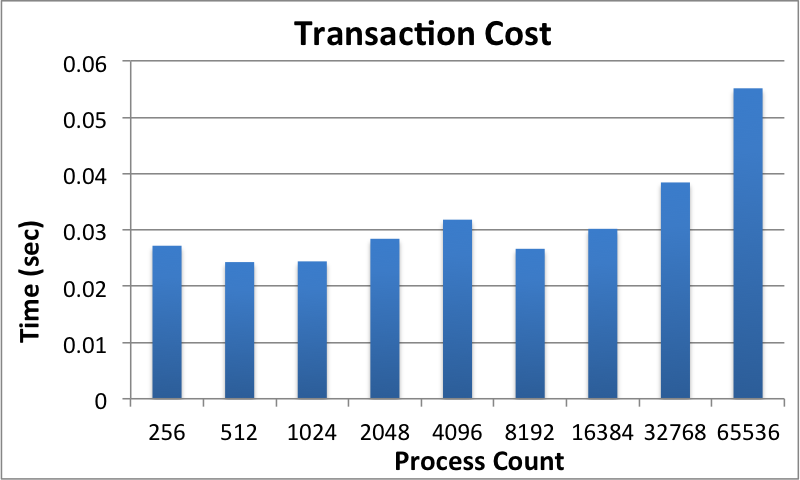
\includegraphics[keepaspectratio=true, width=0.9\columnwidth]{images/performance}
\vspace{-0.15in}
\caption{Total Transaction Overhead}
\label{fig:performance}
\vspace{-0.15in}
\end{figure}

\begin{table}[ht]
    \vspace{-0.15in}
    \centering
    \caption[Scaling Configuration]{Performance Tests Scaling Configuration}
    \bigskip
    \vspace{-0.15in}

    \begin{tabular}{|r|r|r|}
\hline
Processes & \vtop{\hbox{\strut Number of}\hbox{\strut Sub-Coordinators}} & \vtop{\hbox{\strut Processes Per} \hbox{\strut Sub-Coordinator}}\\
\hline
%8 & 2 & 4 \\
%16 & 2 & 8 \\
%32 & 2 & 16 \\
%64 & 2 & 32 \\
%128 & 2 & 64 \\
256 & 2 & 128 \\
512 & 2 & 256 \\
1024 & 4 & 256 \\
2048 & 8 & 256 \\
4096 & 16 & 256 \\
8192 & 32 & 256 \\
16384 & 64 & 256 \\
32768 & 128 & 256 \\
65536 & 256 & 256 \\
\hline
    \end{tabular}
    \label{tab:scaling}
\end{table}

At a a high level, both \DDT and the IOD transactions have the same high-level
design. In both cases, a hierarchical model is employed. In the case of \DDTns,
it is a purely client-side tree using semi-synchronous messaging. The messaging
itself, in the current implementation, uses asynchronous MPI messages. The
synchronous component comes from the timeout mechanism used to detect faults.
It forces a level of coordiation and synchronization for the protocol. For IOD,
it is a server-side tree and fully asynchronous. In both cases, there is a
master in charge of managing the transaction and a collection of workers that
aggregate into the master through second-level leaders. Beyond that, there are
some significant differences. Some of the different choices made by IOD raise
some possible concern.

First, \DDT has a timeout mechanism to detect failures and offer an ability to
recover and clean up the incomplete transactions. IOD's transactions are
asynchronous precluding a relatively simple, short timeout value to detect
failures. Unfortunately, at this point, there is no mechanism in IOD's
transaction handling to detect a fault and clean up any incomplete operations.
While this is intended for phase 2, some initial suggestion on how this might
be handled would give some confidence that the asynchronous approach is viable.

Second, should a transaction on a container not complete, all subsequent
transactions on that container, even if they are complete and correct, will not
be accessible.

Third, in the single leader model, if the process that manages the transaction
were to fail, there is no ability to abort that transaction. The data will not
be made available because the transaction is still listed as in progress. The
problem is that without a way to clean up this failed transaction, no newer
versions of the same container can be made readable. In reality, the single
leader model would ideally outsource the transaction processing to something
like \DDT on the client side. This does not address the failure case though.

Fourth, in the multi-leader model, using a count of client connections to
determine if transaction is complete is problematic.  First, should this be in
an evnironment where lost or repeated network messages are possible, then the
count could be wrong inappropriately. This is a general problem and unlikely
in the current environment, but is a concern on less integrated platforms.
The idea of a count precludes any tracking of expected messages from sources
introducing a potential hole. Second, the aggregation of completion messages
are based on the local aggregation point reporting to the transaction
leader the state.  There is no ability to detect or recover from a failure of
this IOD process that would report to the transaction leader. Third, because a
simple count of participating processes is sent with the beginning of the
transaction, each process is strictly limited to a single output operation.
This precludes a process writing multiple array shards, for example. To put
this in concrete terms, it means that a file could only contain a single,
globally distributed variable (at the root level of HDF5) OR an attribute per
process. If this count actually represents a begin/end transaction pair
instead, it suffers from a lack of accountability for missing object (shard)
writes. All it would indicate is that a process started and ended a transaction
connection. There is no validation that a process has done everything required
of it.

\begin{figure}[ht]
\centering
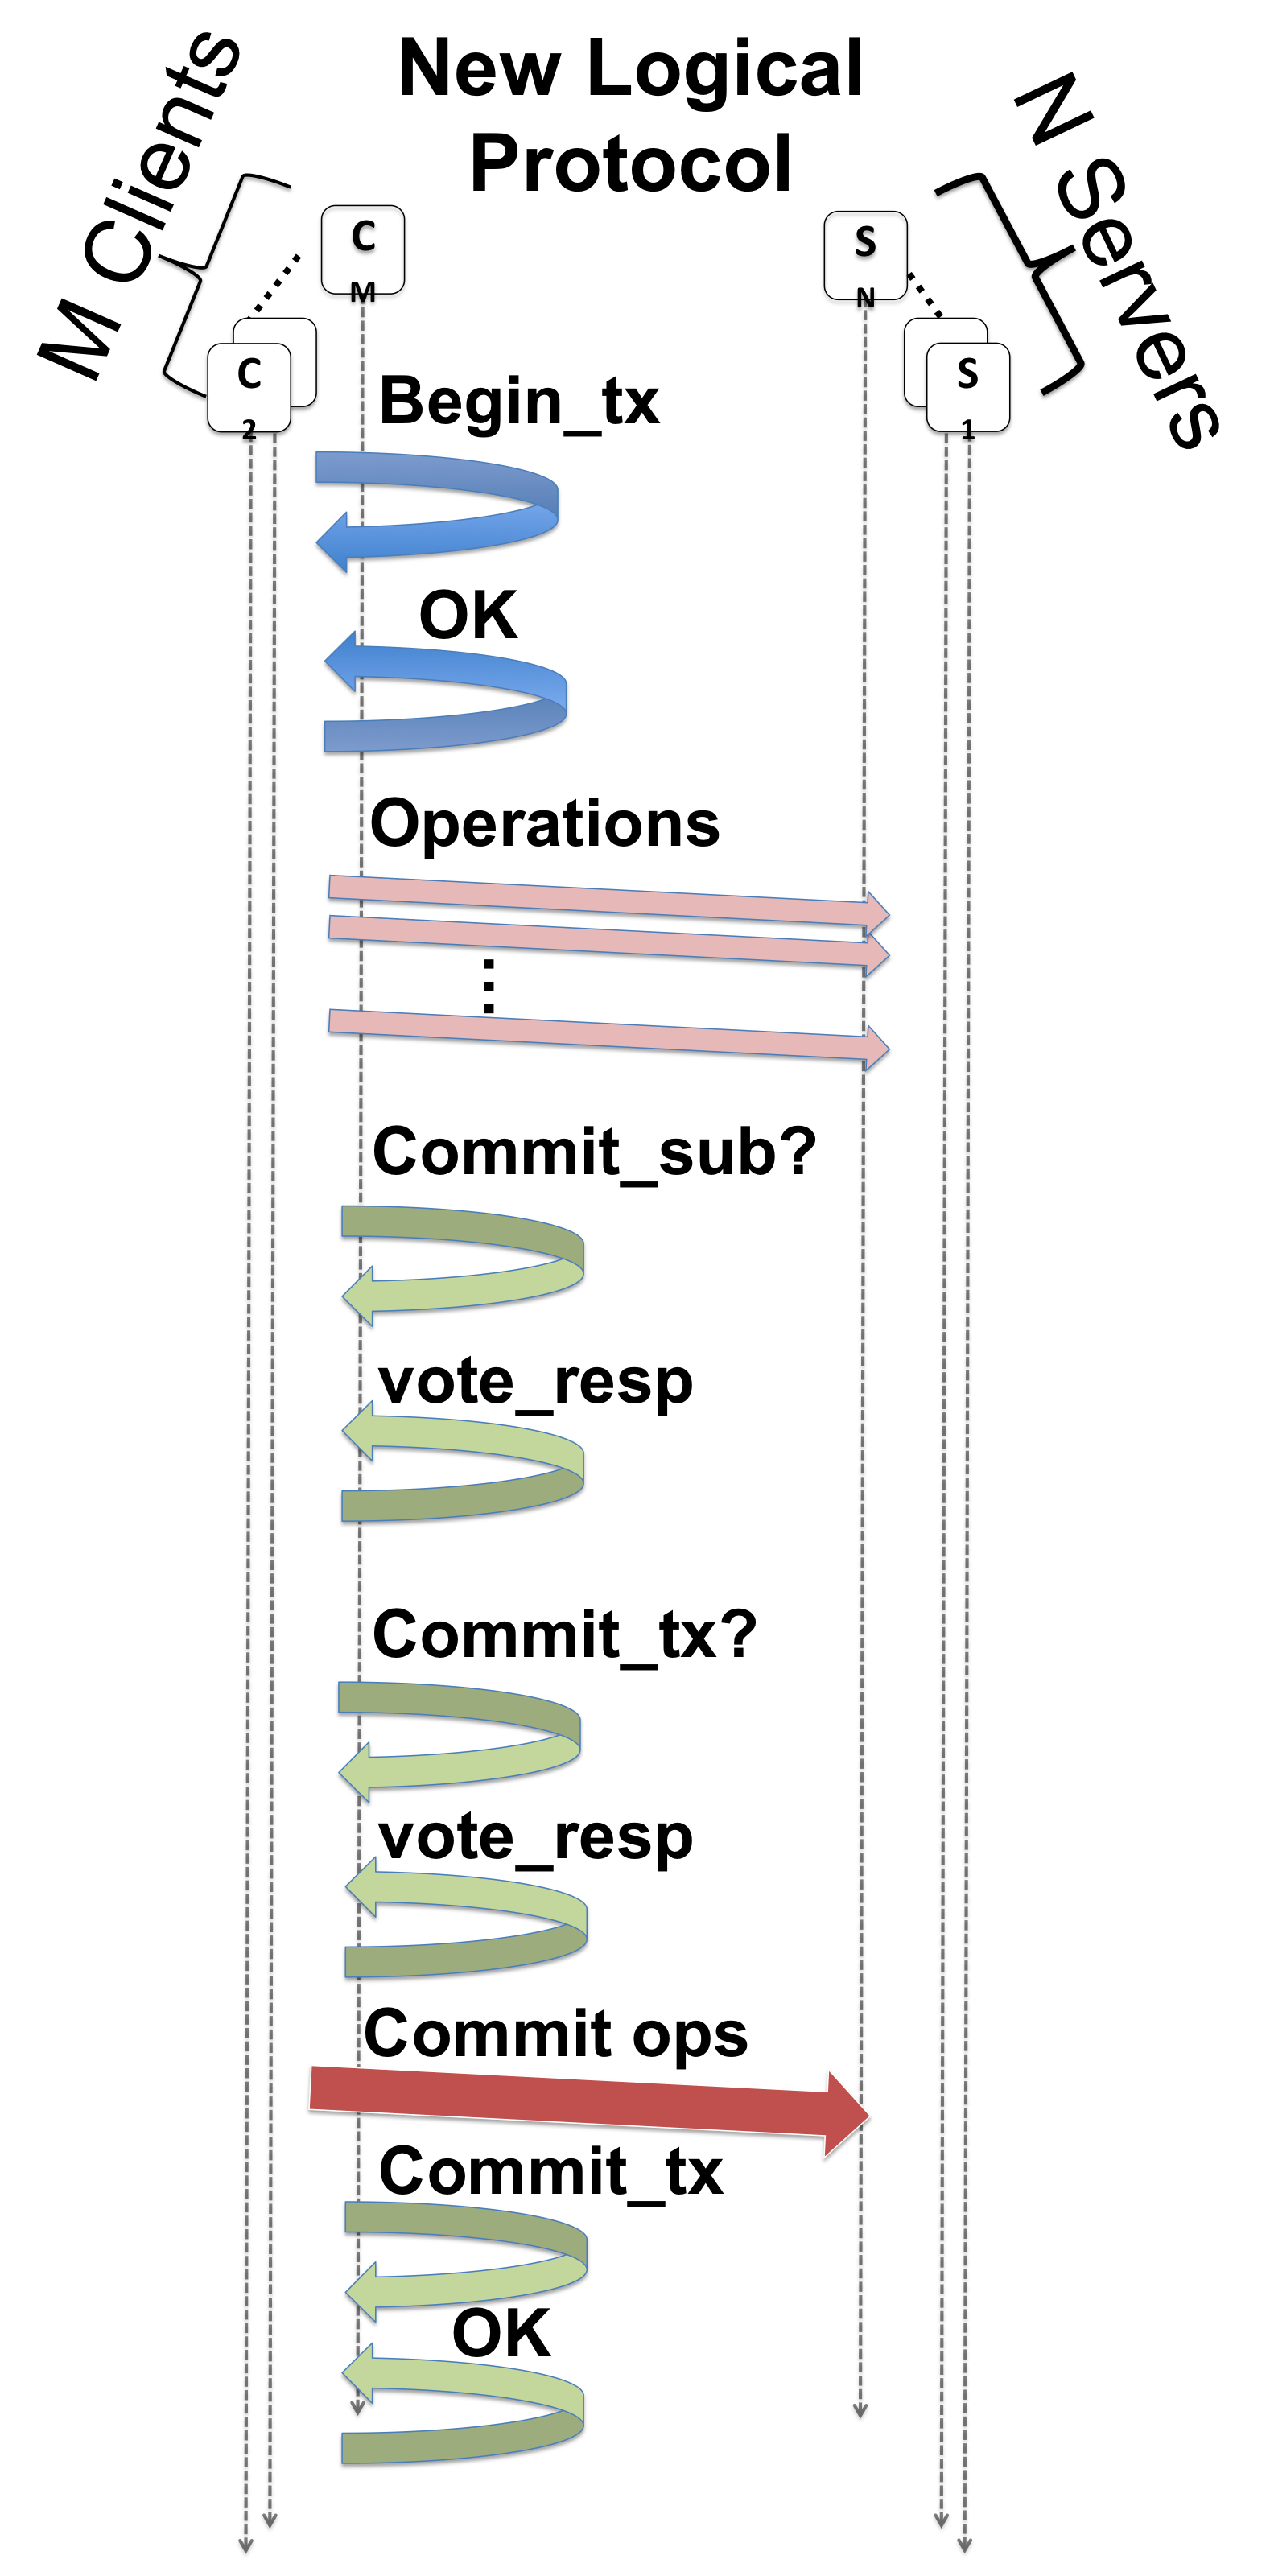
\includegraphics[keepaspectratio=true, width=0.9\columnwidth]{images/optimized-protocol}
\vspace{-0.15in}
\caption{Optimized Protocol}
\label{fig:optimized-protocol}
\vspace{-0.25in}
\end{figure}

\DDT has addressed this count issue in a couple of ways. First, the
sub-coordinators each have a list of processes from which they expect messages.
Should a message be missed, it is noticed and corrective action can be taken.
Second, \DDT has the concept of sub-transactions. The messaging requirements
are illustrated in Figure~\ref{fig:optimized-protocol}.  Sub-transactions
represent finer grained operations than the entire output, \DDT can manage
multiple writes per client by using a sub-transaction to represent the output
for any item to the file (container). Because of how the sub-transactions are
managed, the singleton sub-transactions, ones in which only a single process
participates, must be declared before the transaction begins so that its
existence can be broadcast as part of the begin transaction message. This
ensures there is global knowledge that the sub-transaction is expected.  That
way if the coordinator (transaction leader) fails, which ever process takes
over that role knows to expect a completion message for that sub-transaction or
the overall transaction cannot complete. Global sub-transactions can be defined
at any time since they are a global, synchronized operation broadcasting their
existence. While this additional layer does introduce messaging, the overhead
is quite small.

The advantages of eliminating these messages is not performance as demonstrated
by the performance of \DDTns. Instead, it offers a much less synchronous model
that matches with different programming models, such as Charm++ or other
task-based approaches. Since it can work for the bulk-synchronous model also,
it is a more broadly applicable approach. This assumes that the observed
potential issues can be addressed successfully.

\subsection{Comparision to Other Protocols}
Alternatives, such as Paxos~\cite{Lamport:1998:paxos} algorithms like
ZooKeeper~\cite{Hunt:2010:zookeeper}, suffer from two limitations making them
unsuitable for this environment. First, the distributed servers in Paxos
systems are all distributed copies of each other that eventually become
consistent. Given the scale we wish to address, a single node's memory is
unlikely to be able to hold all of the data necessary for many operations at
scale. They also do not have a guarantee for when consensus will be achieved
without using slower synchronous calls. For the tight timing we wish to
support, we need guarantees of when a consistent state has been achieved.
Second, these systems also all assume that updates are initiated from a single
client process rather than a parallel set of processes as is the standard in
HPC environments.

\DDT uses a second layer of coordination on the client side that greatly
increases the scalability by consolidating messages from clients into unique
sets prior to sending to the overall coordinator. A gossip
protocol~\cite{ganesh:2003:gossip-protocols} may appear sufficient for this
purpose, but the delay of eventual consistency is strictly avoided with this
protocol to ensure guarantees at particular states in the code. For example, if
a failure occurs, the global understanding of the role of all processes is
required in order for effective communication to occur for operations like
creating sub-transactions or voting. In this case, the protocol can offer
stronger statements about consistency than these protocols offer.  These
features offer a way to easily scale the transaction protocol given the
guarantees we wish to offer. The IOD approach does nothing to address these
concerns.

Another effort to offer consistency and data integrity for the ZFS file
system~\cite{zhang:2010:zfs} covers some of the same territory. Instead of a
focus on the processes all having a notion of completion as a transaction, this
work focuses on the integrity of the data movement operations. We view this
work as something that should be considered hand-in-hand with a transaction
approach to ensure the integrity of the movement of the data in addition to the
agreement of processes about the successful completion of a parallel operation.

\section{Optimizations}
\label{sec:optimizations}

THIS MUST BE RECONCILED WITH THE EARLIER TEXT THAT SAYS LARGELY THE SAME THING.

The ability to place functionality at the IOD layer was explored earlier. In
particular, PreDatA~\cite{zheng:2010:predata} demonstrated the advantage to
the approach as well as identified that the placement of the operators should
consider the compute nodes, the staging or burst buffer nodes, or offline
depending on the characteristics of the operation. This consideration should
be incorporated into the design. In particular, one of the key observations
is that the reduced process count may require the entire time between output
operations to perform many of the data processing tasks requested. This was
part of the motivation prompting evaluating placement decisions at the compute
node, in a staging area, or offline. In the case of the IOD design, it forces
a staging area deployment and then shares that staging area across all users
simultaneously. This is unlikely to be useful because of the limited compute
and communication capacity to spare to perform these operations at a bottleneck
in the IO path. The use of a separate staging area to perform these computations
intentionally selects a location separate from the IO path to avoid these
bottlenecks and potential scalability issues.

\section{Broader Design}
\label{sec:summary}

THiS SECTION NEEDS SOME HELP

Consider a shared file system across an HPC data center. The current design
maintains the metadata in the IOD layer localized to a single machine
effectively making the data inaccessible from another platform.

There is a change in definitions between the IOD layer and the DAOS layer.
For the IOD layer, a container is a collection of objects. For the DAOS layer,
a continer is a collection of shards. For the IOD an object may be a shard of
a global array. For DAOS, a shard can host a set of DAOS objects. Having the
same names with locally correct, globally conflicting definitions serves to
confuse how the system should work.

\section{Conclusions}
\label{sec:conclusion}

The Fast Forward Storage and IO Stack project has designed a good first pass at
addressing the requirements for an extreme scale data storage mechanism. The
split between the IOD layer and the DAOS layer offers a fast place for
intermediate data without requiring the overhead of writing to persistent
storage. The envisioned transaction mechanism, while not perfect in the current
form, is another good attempt to address both failures and prevent access to
incomplete or incorrect data by downstream data consumers. Integrated with the
IOD functionality, this concept represents the concensus approach for what will
be required.

The partial metadata management incorporated into the IOD layer and the lack of
consideration for how to handle and recover from failures are oversights in the
current documents. It is our undertanding that these will be addressed in the
next phase and we hope to help inform that effort with our experiences.

We hope that the efforts made in the \DDT project and other efforts to explore
the requirements for this space, along with the analysis presented in this
paper will prove useful for the next phase of the Fast Forward project.

\section{Acknowledgements}

\includegraphics[scale=0.07]{logos/doe_logo}

\includegraphics[scale=0.30]{logos/snl_logo}

\includegraphics[scale=0.35]{logos/nnsa_logo}
Sandia National Laboratories is a multi-program laboratory managed and operated
by Sandia Corporation, a wholly owned subsidiary of Lockheed Martin
Corporation, for the U.S. Department of Energy's National Nuclear Security
Administration under contract DE-AC04-94AL85000.

\bibliographystyle{abbrv}
\bibliography{paper}

\vfill\eject

\end{document}
